\documentclass{standalone}
\usepackage{tikz}
\usetikzlibrary{angles}
\usetikzlibrary{quotes}

\usetikzlibrary{calc,angles,positioning}
\usepackage{amsmath,tkz-euclide}
\usetkzobj{all}

\begin{document}

%x description="draw an elliptic slice"
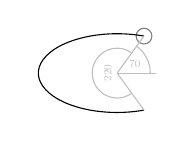
\begin{tikzpicture}
\draw[gray] (0,0) circle (0.1);
%x step={
\draw 
	(0,0) arc 
		[x radius=1, y radius=0.5, 
		start angle=70, delta angle=220] 
	% or 
	(0,0) arc 
		[x radius=1, y radius=0.5,
		start angle=70, end angle=290] % ignores delta angle
	;
%x }

	\begin{scope}[lightgray]
		\path (0,0) 
			coordinate (start) 
			arc [x radius=1, y radius=0.5, start angle=70, end angle=90] 
			++(0,-0.5) 
			coordinate (center) ;
		\path (0,0)
			arc [x radius=1, y radius=0.5, start angle=70, end angle=290]
			coordinate (end);
		\draw (center) -- (0,0);
		\draw (center) -- (end);
		\draw (center) -- ++(0.5,0) coordinate (a);
		
		\draw pic [draw, "220" {xshift=2, rotate=90, scale=0.4}, angle radius=9] {angle = start--center--end};
		\draw pic [draw, "70" scale=0.4, angle radius=12] {angle = a--center--start};
	\end{scope}

\end{tikzpicture}



\end{document}
